\documentclass[10pt,a4paper]{report}

\usepackage[utf8]{inputenc}
\usepackage{amsmath}
\usepackage{amsfonts}
\usepackage{amssymb}
\usepackage{graphicx}
\usepackage{color}
\usepackage{enumitem}
\usepackage[top=1cm, bottom=2cm, left=2cm, right=2cm]{geometry}

\usepackage{fancyhdr}
\pagestyle{fancy}

\fancyhead{}
\fancyfoot{} 
\lhead{
\includegraphics{../Logo/logoKNKMini.jpg} \hspace{0.1cm} Kould Not Konect  \hspace{0.4cm} \vline}
\chead{Document de Conception Générale}
\rhead{Kould Not Share}
\rfoot{\thepage}

\author{Kevin BASCOL, Kevin LAOUSSING, Nicolas REYNAUD}
\title{Document de conception générale}
\date{3 Novembre 2014}

\makeatletter
\renewcommand{\thesection}{\@arabic\c@section}
\makeatother

\begin{document}

\makeatletter
	\begin{titlepage}
	
	\begin{figure}
		\begin{minipage}[c]{.46\linewidth}
		\end{minipage} \hfill
		\begin{minipage}[c]{.20\linewidth}
			\begin{center}
				
\includegraphics{../Logo/logoKNK.jpg}\\
				{\large Kould Not Konect}
			\end{center}
		\end{minipage}
	\vspace{1cm}
	\end{figure}
	
	\centering
		{
		\hrule height 2pt
		\vspace{0.7cm}
		\Huge \textbf{\@title}}\\
		\vspace{0.7cm}
		\hrule height 2pt
		\vspace{1.5cm}
		{\LARGE  Projet \textbf{Kould Not Share} v1.0}
		
		\vfill
		
		\begin{tabular}{|c|c|c|}
			\hline
			Version & Date & Description\\
			\hline
			V.1 & 03/11/14 & Première version de la conception générale\\
			\hline
			 & & \\
			\hline
			 & & \\
			\hline
		\end{tabular}\\
		\vspace{1cm}
		\@author\\
		\end{titlepage}
\makeatother
\setcounter{secnumdepth}{5}
\setcounter{tocdepth}{5}
\renewcommand{\contentsname}{Sommaire}
\begingroup\makeatletter
\def\@makeschapterhead#1{%
  {\parindent \z@ \raggedright
    \normalfont
    \interlinepenalty\@M
    \Huge \bfseries  #1\par\nobreak
    \vskip 20pt% <---- à réduire pour avoir plus de place
  }}\makeatother
\tableofcontents
\endgroup
\thispagestyle{empty}
\setcounter{page}{0}
\newpage

\newgeometry{top=2cm, bottom=2cm, left=2cm, right=2cm}



\section{Objectif du document}
Ce document présente la conception logicielles et matérielles de la version 1.0 du projet Kould Not Share de l'entreprise Kould Not Konnect. Les responsables de ce projet sont Nicolas Reynaud, Kevin Laoussing et Kevin Bascol.

\section{Décomposition du système en modules (architecture)}

\subsection{Schéma du système}
\begin{center}
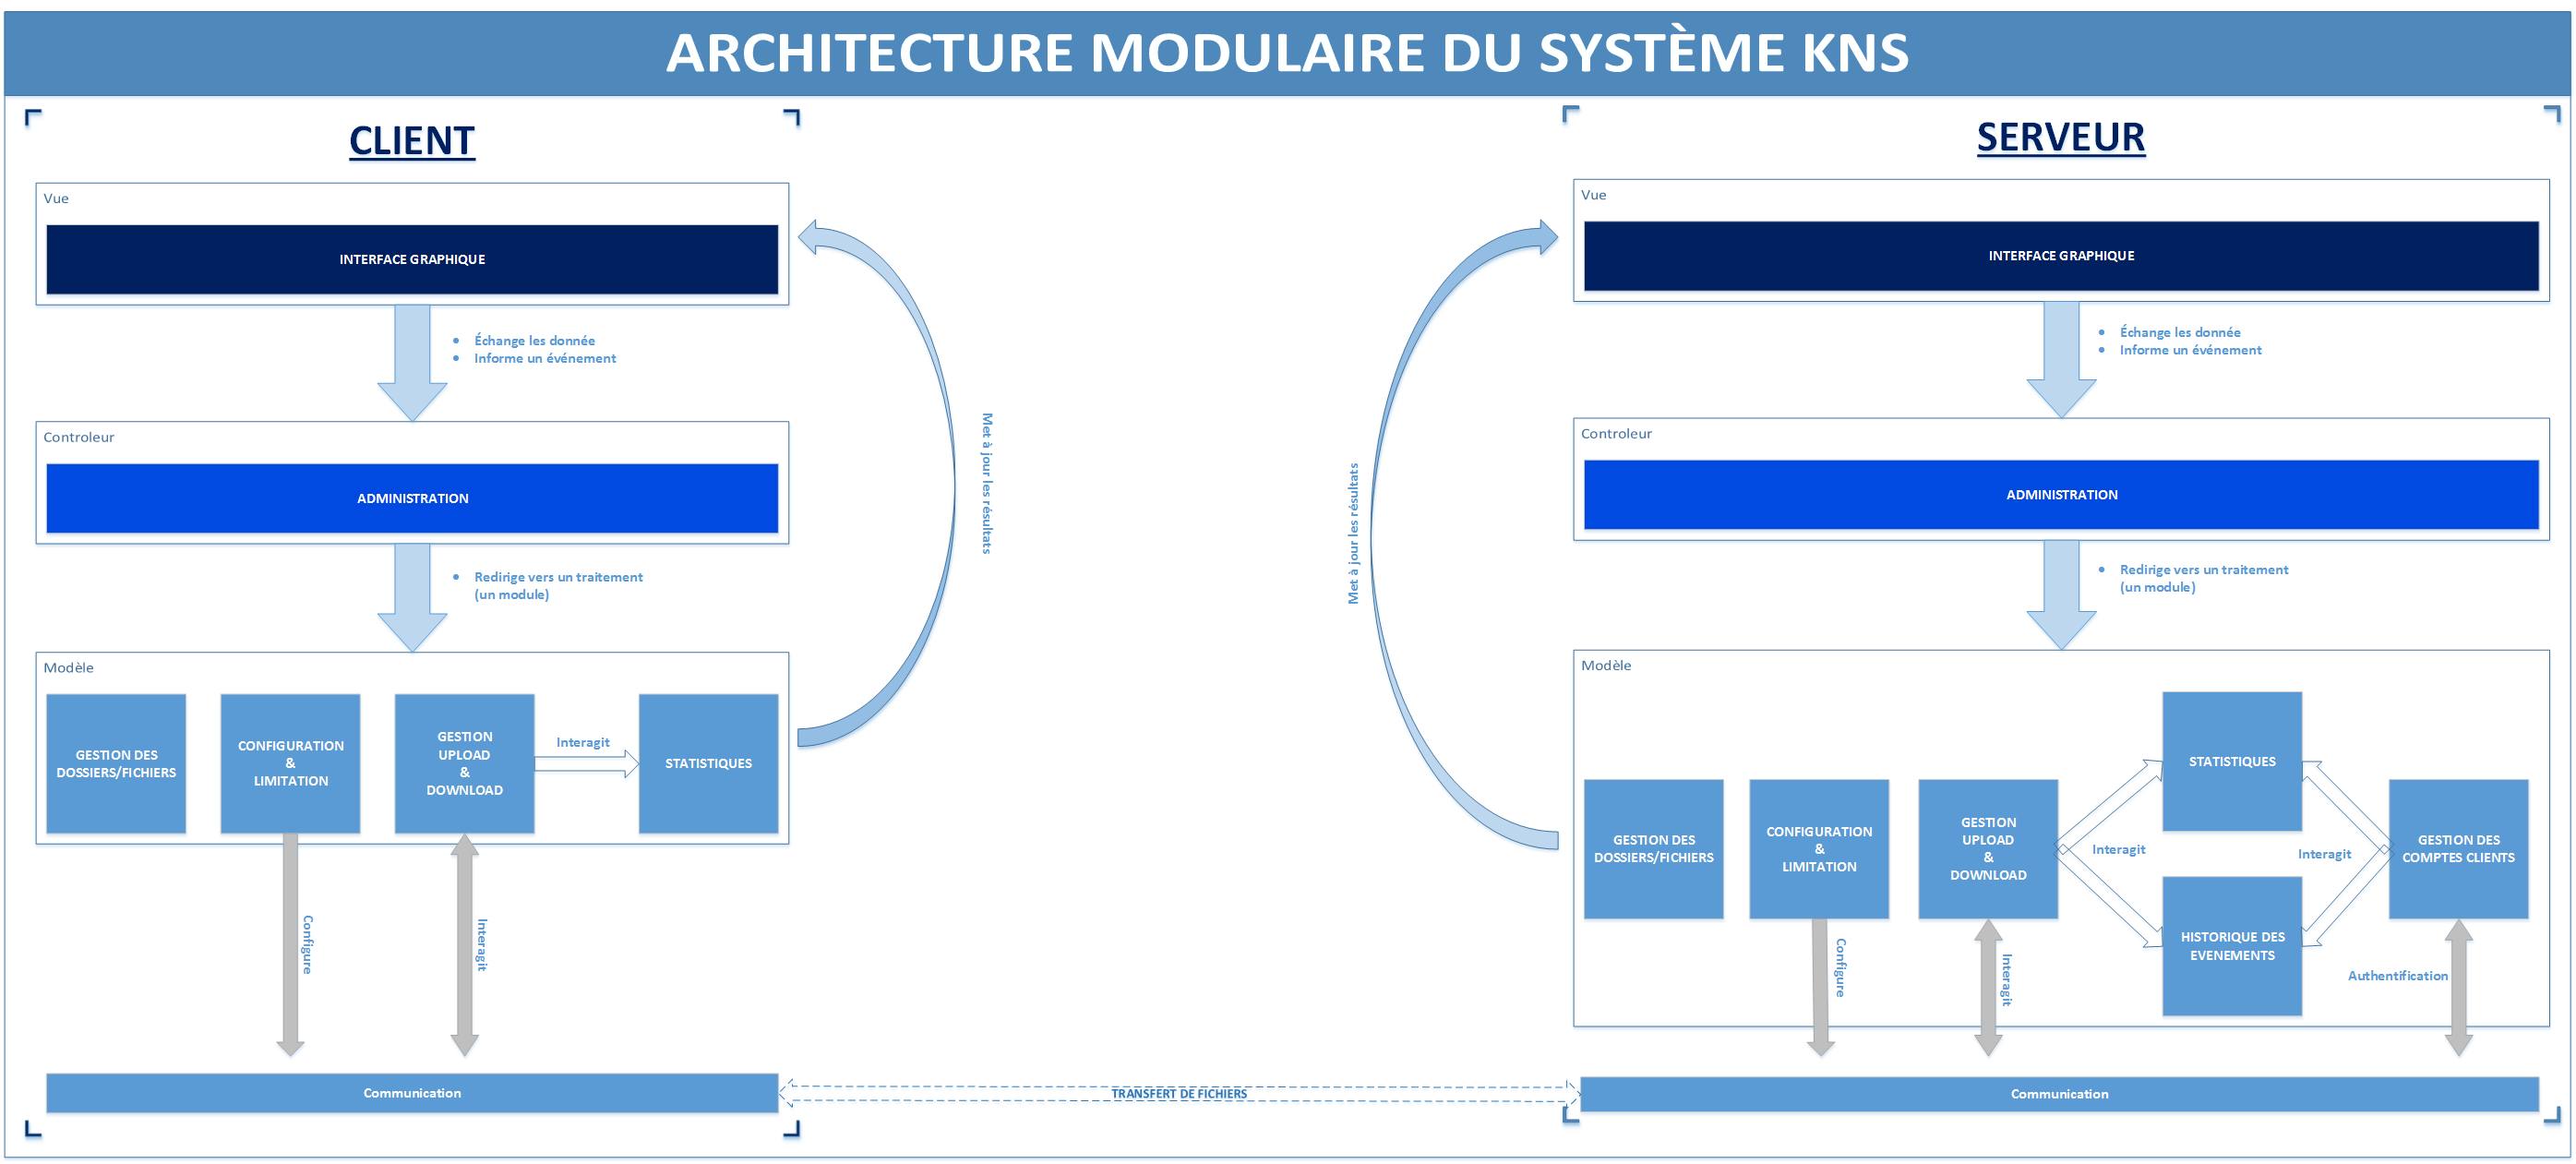
\includegraphics[scale=0.23]{Ressources/modules_KNS.png}
\end{center}
(cf Annexe)
\subsection{Description des modules}

\subsubsection{Modules Client}

	\paragraph{Module de l'interface graphique}
	
	
	\paragraph{Module d'administration}
	
	
	\paragraph{Module de gestion de dossier}
	
	
	\paragraph{Module de configuration et limitation}	
	
	
	\paragraph{Module de upload/download}
	
	
	\paragraph{Module de statistiques}
	
	
	\paragraph{Module de communication}


\subsubsection{Modules Serveur}

	\paragraph{Module de l'interface graphique}
	
	
	\paragraph{Module d'administration}
	
	
	\paragraph{Module de gestion de dossier}
	
	
	\paragraph{Module de configuration et limitation}	
	
	
	\paragraph{Module de upload/download}
	
	
	\paragraph{Module de statistiques}

	
	\paragraph{Module des historiques des événements}
	
	
	\paragraph{Module de gestion des comptes clients}
	
	
	\paragraph{Module de communication}

\section{Définition des principales structures de données}

\subsection{Structures de données}

\subsection{Interactions entre les structures de données} %<--- diagramme de séquence ?%

\newpage
\section{Annexe}

\subsection{Architecture modulaire du système KNS}
	\begin{center}
	\rotatebox{270}{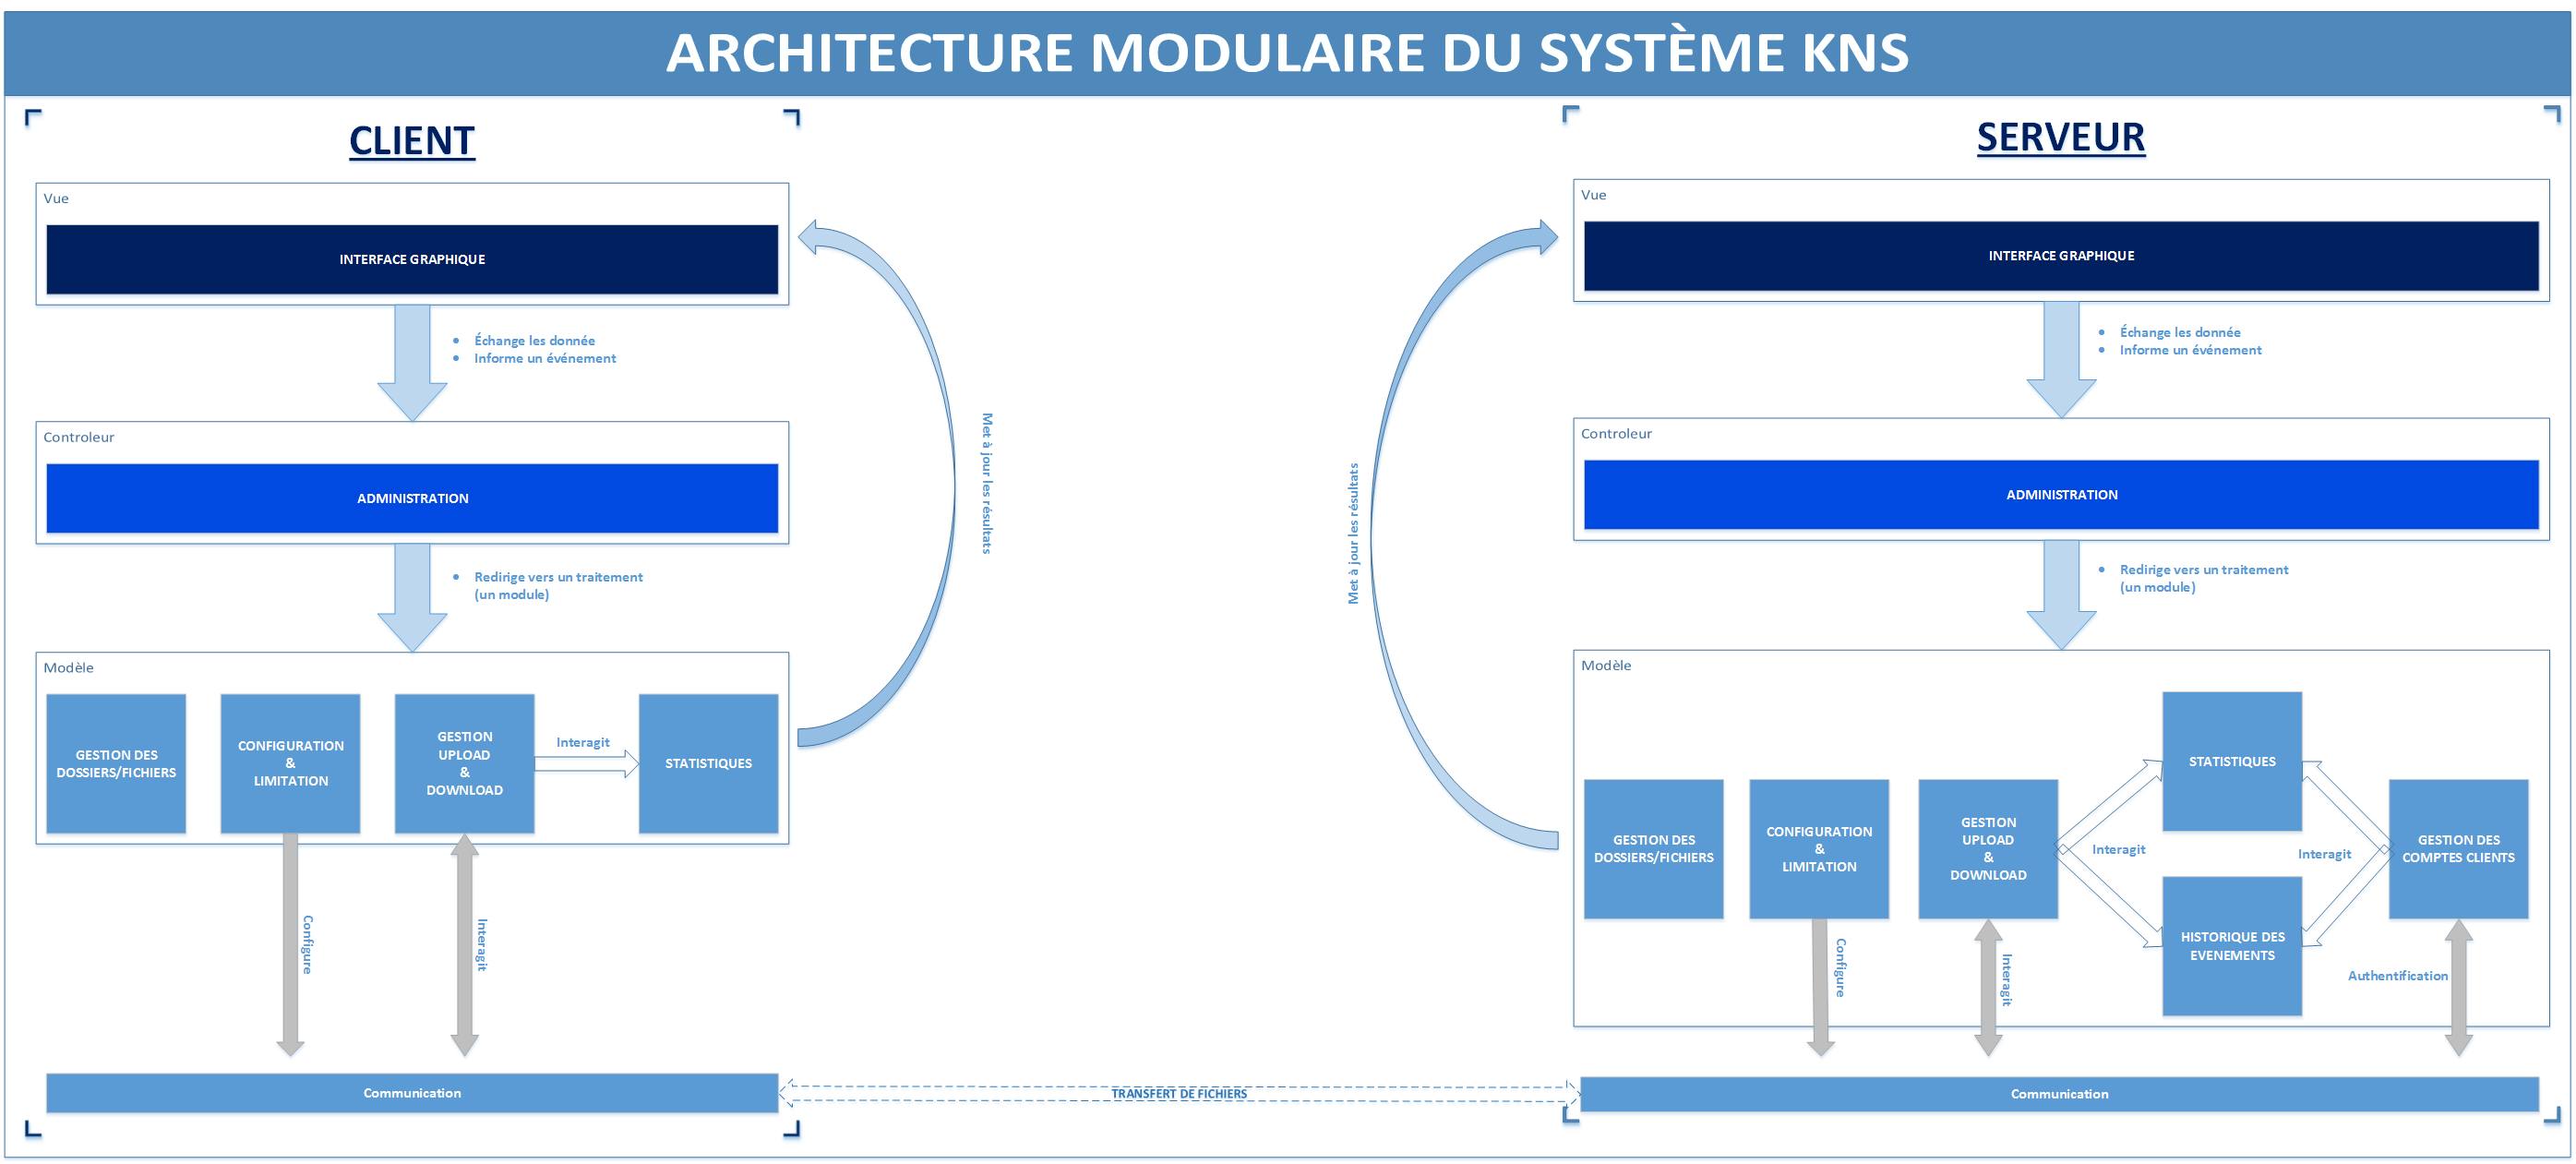
\includegraphics[scale=0.35]{Ressources/modules_KNS.png}}	
	\end{center}
\end{document}